% !TeX root = ./Diplomarbeit.tex
% config.tex

\author{Albrecht Naumann}
\title{Diplomarbeit}

\documentclass [
    a4paper,
    12pt,
    oneside
] {scrreprt}
% TODO: wenn notwendig, noch Fußnotengröße setzen -2pt

%
% Language
%
\usepackage[utf8]{inputenc}
\usepackage[T1]{fontenc} % europäische Zeichen

%
% Document Format
%
\usepackage{geometry}
\usepackage{graphicx}
\usepackage{subcaption}
\usepackage{float}

\usepackage[font=small,labelfont=bf]{caption}

% default pdf version 1.5 => changed to 1.7
\pdfminorversion=7

% Ränder
\geometry{includeheadfoot, top=2cm, bottom=2cm, left=3cm, right=2cm}
%Zeilenabstand
\renewcommand{\baselinestretch}{1.5}\normalsize
% Arial
% \renewcommand{\familydefault}{\sfdefault}
\tolerance=200
\emergencystretch=1em % Tolleranz

% Titelformat
% \usepackage{titlesec}
% \titleformat{\chapter}[block]
%   {\normalfont\LARGE\bfseries}{\thechapter.}{.5em}{\LARGE}
% \titlespacing*{\chapter}{0pt}{0pt}{1em}
% \titleformat*{\section}{\large\bfseries}
% \titlespacing*{\section}{0pt}{1em}{1em}
% \titleformat*{\subsection}{\normalfont\bfseries}

% global packages
%
\usepackage{url}
\usepackage[ampersand]{easylist}
\usepackage[utf8]{inputenc}
\usepackage{scrhack}
%
% references
%
\usepackage[babel,german=guillemets]{csquotes}
% \usepackage[style=authoryear]{biblatex}
\usepackage[
    backend=biber, 
    style=authoryear, 
    maxnames=2,
    minnames=1,
    isbn=false,
    doi=false,
]{biblatex} %biblatex mit biber laden
% \ExecuteBibliographyOptions{
%   sorting=nyt, %Sortierung Autor, Titel, Jahr
%   bibwarn=true, %Probleme mit den Daten, die Backend betreffen anzeigen isbn=false, %keine isbn anzeigen
%   url=false %keine url anzeigen
% }

\DefineBibliographyStrings{ngerman}{ 
   andothers = {et\addabbrvspace al\adddot},
   andmore   = {et\addabbrvspace al\adddot},
}

\addbibresource{literatur.bib}

\usepackage[table]{xcolor}
\definecolor{lstgrey}{rgb}{0.95,0.95,0.95}

% Code-Snippets 
\usepackage{listings}
\lstset{
    numbers=none, 
    numberstyle=\tiny,
    numbersep=5pt, 
    stepnumber=2, 
    frame=single,
    backgroundcolor=\color{lstgrey},
    basicstyle=\footnotesize\ttfamily,
    breaklines=true,
}

% DIR-Tree
\usepackage{dirtree}

% item list
%
\usepackage{paralist}
\renewcommand{\labelitemi}{$\bullet$}
\renewcommand{\labelitemii}{$\circ$}
\renewcommand{\labelitemiii}{$\cdot$}
\renewcommand{\labelitemiv}{$\ast$}

\usepackage{chngcntr} % => \counterwithin{figure}{chapter}
\counterwithin{figure}{chapter}

\usepackage[ngerman]{babel}
\addto\captionsngerman{
  % \renewcommand{\figurename}{Abbildung}
  % \renewcommand{\tablename}{Tab.}
  % \renewcommand{\lstlistingname}{Listing}
}
\renewcommand{\lstlistlistingname}{Abbildungsverzeichnis}%  List of Listings -> Abb.

\usepackage{amsmath}

% sonstiges
\usepackage{framed}
\usepackage{mathabx}

\usepackage{multicol}

% table
\usepackage{longtable}
\usepackage{tabularx,  multirow}
\usepackage{ltxtable}
 
% frame
\usepackage{efbox,graphicx}
\efboxsetup{linecolor=black,linewidth=.2pt}

\newcounter{magicrownumbers}
\newcommand\rownumber{\stepcounter{magicrownumbers}\arabic{magicrownumbers}}
\newcommand\rownumbereset{\setcounter{magicrownumbers}{0}}
% mute warnings
\usepackage{silence}
\WarningFilter{latex}{Writing or overwriting file}
\WarningFilter{latex}{File `Diplomarbeit_Albrecht_Naumann-storetable.tex' already exists on the system.}
%
% PDF output
%
\usepackage[
    bookmarks=true,         % show bookmarks bar?
    unicode=false,          % non-Latin characters in Acrobat’s bookmarks
    pdftoolbar=true,        % show Acrobat’s toolbar?
    pdfmenubar=true,        % show Acrobat’s menu?
    pdffitwindow=false,     % window fit to page when opened
    pdfstartview={FitH},    % fits the width of the page to the window
    pdfauthor={Albrecht Naumann},     % author
    pdfnewwindow=true,      % links in new PDF window
    colorlinks=false,       % false: boxed links; true: colored links
    hidelinks
    % linkcolor=red,          % color of internal links (change box color with linkbordercolor)
    % citecolor=green,        % color of links to bibliography
    % filecolor=magenta,      % color of file links
    % urlcolor=cyan           % color of external links
]{hyperref}


% \chapter*{Glossar}
% \addcontentsline{toc}{chapter}{Glossar}
% \begin{description}
%     \item[Freedesign-Editor] Eine Software zur Gestaltung von Druckprodukten, die von der Onlinedrucker Unitedprint.com SE entwickelt wird und in den Onlineshops des Unternehmens bereitgestellt wird.
%
%     \item[Unit-Testing] Unit-Testing ein Vorgehen zum Testens des Quelltextes einer Software.
% \end{description}

\longnewglossaryentry{Freedesign-Editor}{name=Freedesign-Editor}{Eine Software zur Gestaltung von Druckprodukten, die von der Onlinedrucker Unitedprint.com SE entwickelt wird und in den Onlineshops des Unternehmens bereitgestellt wird.}

\longnewglossaryentry{Unit-Testing}{name=Unit-Testing}{Unit-Testing ein Vorgehen zum Testens des Quelltextes einer Software.}

\longnewglossaryentry{Unit-Test}{name=Unit-Test}{Der Unit-Test ist ein Test zur Prüfung von Quelltext.}


\begin{document}
    % % Deckblatt.tex
% TODO: final anpassen
\begin {titlepage}
\begin {center}
% 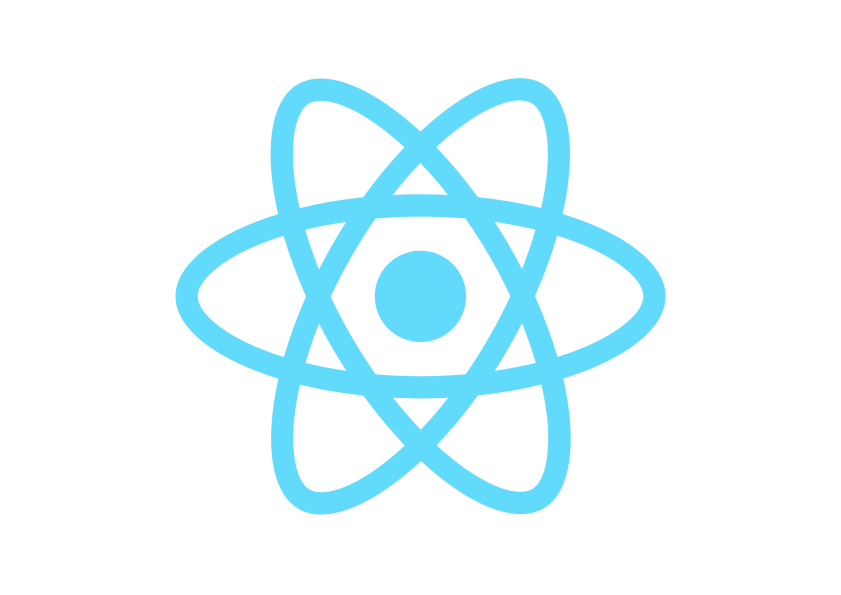
\includegraphics [width=1.0\linewidth] {pics/logo}
\small{
	%\begin{tabular}{c}
	Westsächsische Hochschule Zwickau \\
	FAKULTÄT  WIRTSCHAFTSWISSENSCHAFTEN\\
	\vspace{7pt}
	in Kooperation mit\\
	\vspace{7pt}
	media project Institut für IT-und Managementtechnologien gGmbH Dresden\\
    berufsbegleitender Studiengang Informatik (Diplom FH)\\
    und\\
    Unitedprint SE\\
	%\end{tabular}
}
\vspace{50pt}

\LARGE{\textbf{Diplomarbeit}}

\vspace{8pt}
\Large{\textbf{vorgelegt von}}
\Large{\textbf{Herrn Albrecht Naumann}}
\end{center}
\vspace{10pt}
\paragraph{Thema:}
\large{
\begin{center}
% TODO: Thema
\end{center}
}
\paragraph{Zeitraum:}
\large{
\begin{center}
% TODO: Zeitraum
\end{center}
}
\end{titlepage}
  TODO: Deckblatt aktivieren
    \pagenumbering{roman}
    \tableofcontents

    \listoffigures
    % TODO:Tabellenverzeichnis

    \pagenumbering{arabic}
    \clearpage % reset page count
    % \printglossaries

    \input{chapter/Einführung}
    % Grundlagen.tex
\chapter{Grundlagen}
\section{Der FreeDesign-Editor}
\label{Der FreeDesign-Editor}
\subsection{Funktionsbeschreibung}
Der, durch Unitedprint bereitgestellte, Webshop \emph{easyprint.com} bietet Kunden die Möglichkeit Druckprodukt online zu gestaltet und im Anschluss zu bestellen. Für die Gestaltung der Produkte wurde unternehmenintern die Webanwendung \emph{FreeDesign} entwickelt, welche beständig gepflegt und weiterentwickelt wird. Die Anwendung ist eine Single-Page-Webanwendung, welche in der Programmiersprache TypeScript, sowie unter der Verwendung von \emph{ReactJS} und \emph{Redux} entwickelt wurde. 

Basierend auf Flanagan (\citeyear[S. 497]{Flanagan2006}) wird als Single-Page-Webanwendung ein Webanwendung bezeichnet die auf der Ajax-Technologie basiert und ihre Inhalt per JavaScript aktualisiert und nicht durch das neu Laden der Anwendung. 

Mit hilfe des Editor kann eine große Vielzahl von Druckprodukten gestaltet werden, wobei das Portfolio verschiedenste Produktgruppen, wie Bürozubehör, Textilien oder Werbematerialien, abdeckt. Zur Gestaltung eines Designs bietet der Editor die Möglichkeit der Nutzung eigener Text und Bilder sowie das Verwenden verschiedenster geometrischer Formen. Alle Element können umfangreich geometrisch und grafische bearbeitet werden. Um einen optimalen Gestaltungsprozess zu ermöglichen, kann die Produktdarstell auch wärend der Gestaltung vergrößert, verschoben oder rotiert werden. Weiterhin stehen auch Hilfwerkzeuge wie Lineal oder Hilflinien zur Verfügung. 

Die Nutzer haben auch die Möglichkeit Designs als Entwürfe zu speicheren und zu einem späteren Zeitpunkt zu öffnen.

\begin{figure}[H]
    \centering
    \efbox{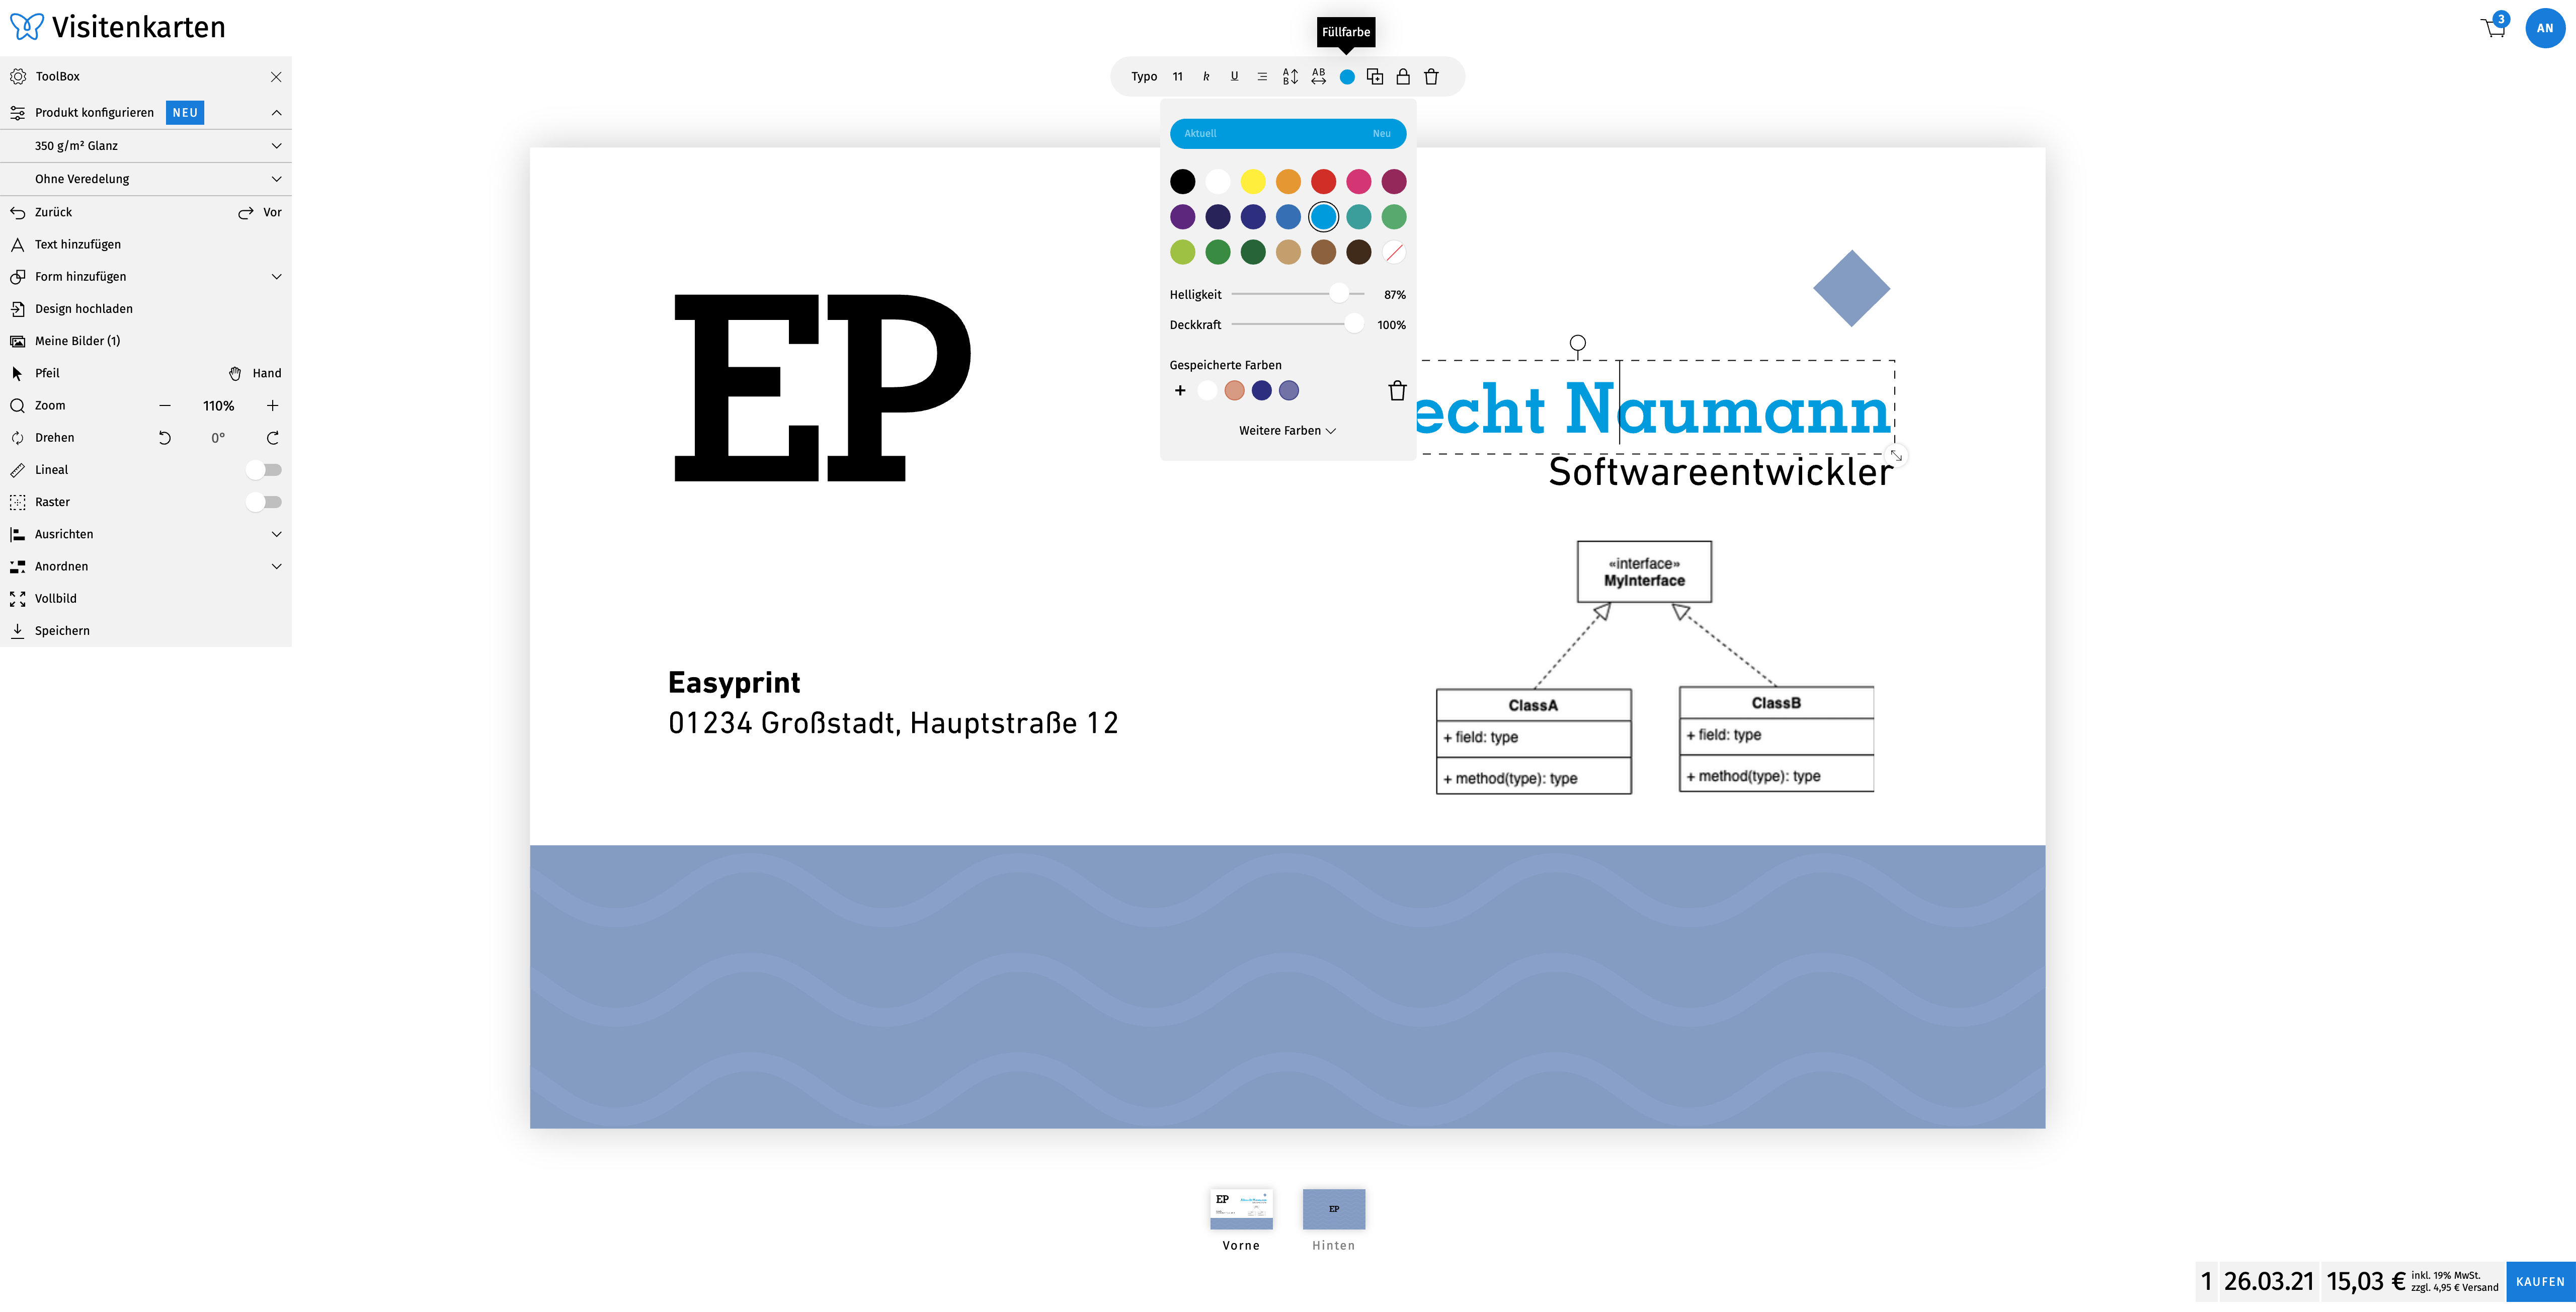
\includegraphics[width=.98\textwidth]{chapter/freedesign/Screenshot-Freedesign.png}}
    \caption{Ein Bildschirmfoto des FreeDesign-Editor}
    \label{fig:Der FreeDesign-Editor}
\end{figure}

\subsection{Designvorlagen}

\begin{figure}[H]
    \centering
    \efbox{\includegraphics[width=.98\textwidth]{chapter/freedesign/Screenshot-Designseite.png}}
    \caption{Ein Bildschirmfoto der Designübersichtseite für Visitenkarten}
    \label{fig:Designuebersichtseite}
\end{figure}

\begin{figure}[H]
    \centering
    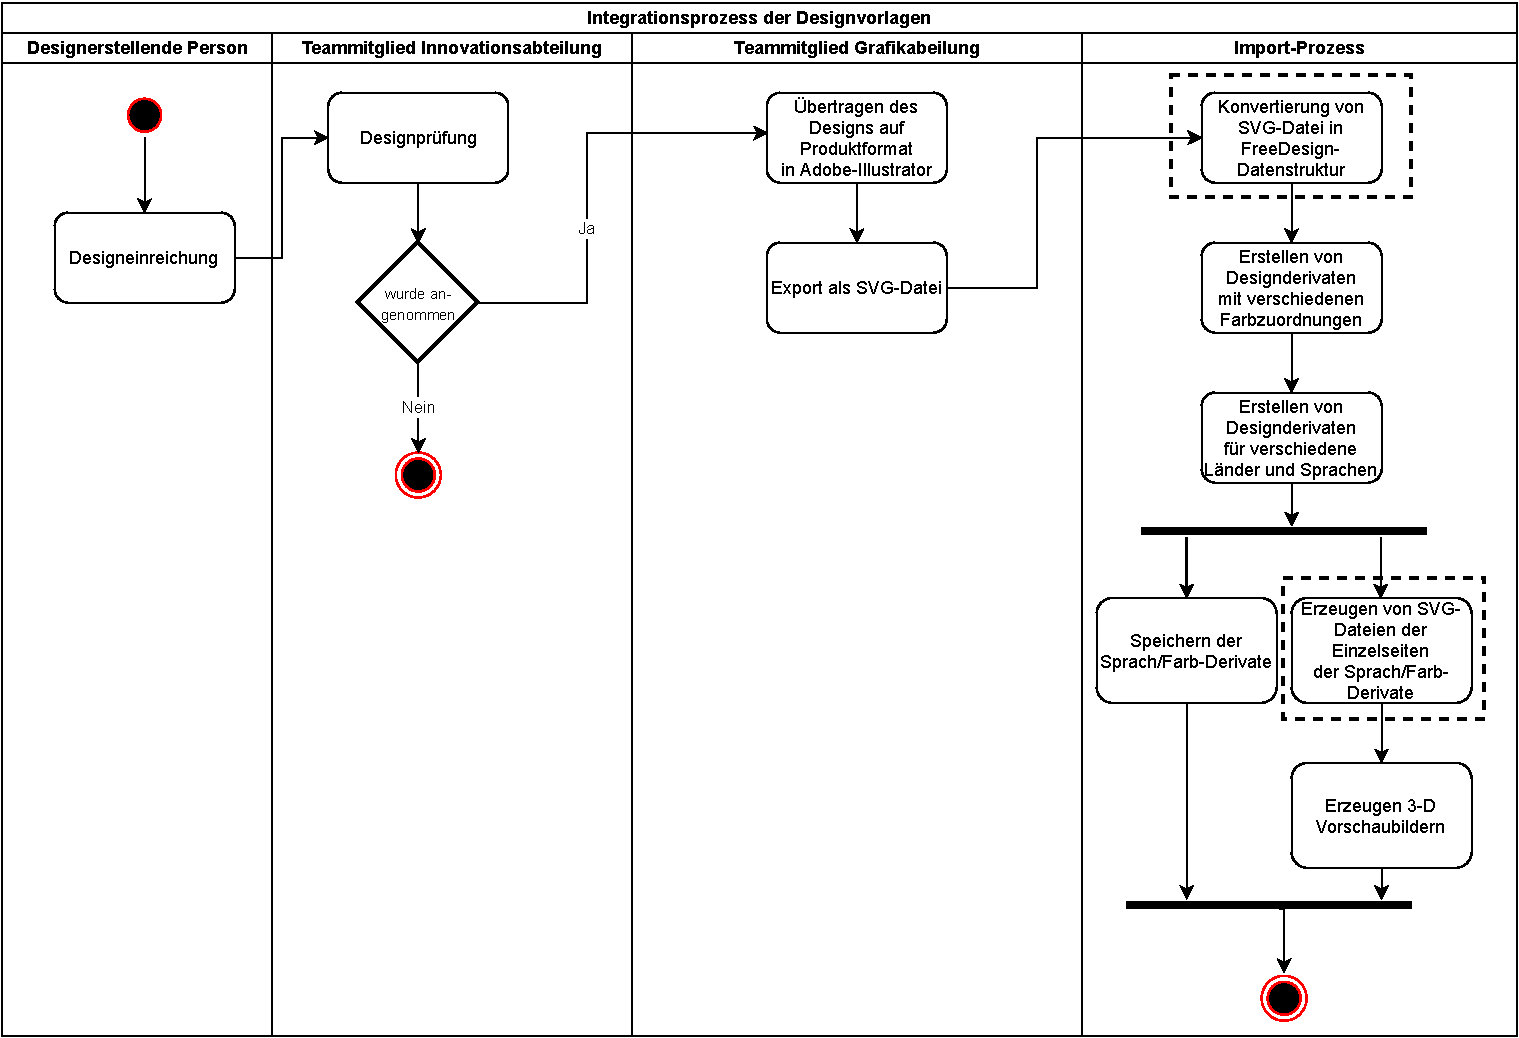
\includegraphics[width=.98\textwidth]{diagrams/Freedesign-Vorlagenerstellung.pdf}
\caption{Prozessbeschreibung der Vorlagenerstellung}
\label{fig:Vorlagenimport}
\end{figure}

\subsection{Bestellablauf}
%TODO: => Auf Team eingehen


\section{Unit-Testing}
\subsection{Definition}
Anlehnend an Osherove (\citeyear[S. 34]{Osherove2015}) ist ein \gls{Unit-Test} ein Stück Quelltext, welcher automatisch einen isolierten Baustein, das Testobjekt, einer Software ausführt. Dabei kann das Testobjekt ein Skript, eine Funktion, ein Modul oder bei objektorientierten Sprachen eine Klasse sein. Wichtig ist, dass das Testobjekt abgeschlossen ist. Nach der Ausführung prüft der Unit-Test das Ergebnis, welches vom Testobjekt erzeugt wurde. Entspricht das Ergebnis den vom Test definierten Erwartungen, wird das Testergebnis als erfolgreich gekennzeichnet, andernfalls wird es als negativ gekennzeichnet.
Das Testergebnis ist konsistent, solange die Logik des Testobjektes nicht geändert wird.

\subsection{Anforderungen an Unit-Tests}
\subsubsection*{Unabhängigkeit der Unit-Tests}
Die Entwicklung einer Software sollte von regelmäßigen Ausführungen und Erweiterungen der Unit-Tests durch die Entwickler begleitet sein. Damit die Tests regelmäßig von den Entwicklern ausgeführt werden, sollte ihre Ausführung Millisekunden bis maximal wenige Sekunden lang dauern. Andernfalls würde die Akzeptanz der Tests bei den Entwicklern gesenkt. Die Ausführung der Tests sollte auch die Entwicklungsarbeit nicht unterbrechen oder gar blockieren. Um dies zu gewährleisten, ist es wichtig, dass die Unit-Tests unabhängig von ihrer Umgebung ausführbar sind und nicht aufeinander aufbauen \autocite[vgl.][S. 19]{Springer2015}. Das bedeutet, dass keine Datenbankverbindung oder Verbindung zu anderen Systemen bestehen darf. Diese Verbindungen würden es notwendig machen, die Testumgebung zu konfigurieren und würden die Testsausführung verlangsamen oder auch stören. Das Testen mit Datenbankenverbindungen und weiteren externen Abhängigkeiten wird den Integrationstests und den Systemtests überlassen.
Durch die schnelle Ausführbarkeit muss der Entwickler auch nicht jedesmal die gesamte Applikation starten, um seine Arbeit zu prüfen.
\subsubsection*{Leichte Verständlichkeit}
Eine weitere wichtige Anforderung an Unit-Tests ist, dass sie leicht verständlich programmiert sind und sich somit jedem Entwickler, der im Projekt involviert ist, innerhalb weniger Minuten erschließen \autocite[vgl.][224]{Osherove2015}. Somit können eventuelle Fehlfunktionen, die zu fehlerhaften Unit-Tests führen, schnell vom Entwickler erfasst werden.
Das hilft den involvierten Entwicklern den Quelltext der Software leichter zu verstehen. Unit-Tests können somit auch als Teil der Softwaredokumentation für die Entwickler gesehen werden \autocite[vgl.][19]{Springer2015}.


Da Software aus einer Vielzahl von Funktionen und Funktionalitäten besteht, ist ebenfalls mit einer Vielzahl von Unit-Tests zu rechnen. Aus diesem Grund sollten die Tests von Anfang an in einer sinnvollen Struktur angelegt werden und mit Techniken ausgestattet sein, welche die Wartung der Tests möglichst gering hält.

\subsubsection*{Vermeidung von Logik in den Unit-Tests}
Innerhalb der Unit-Tests sollte auf Logik verzichtet werden \autocite[vgl.][197]{Osherove2015}. Diese führt nicht nur zur schweren Verständlichkeit der Tests, sondern macht die Unit-Tests selber anfällig für Fehler.

\subsection{Mehraufwand durch das Erstellen von Unit-Tests}
Das Erstellen von Unit-Tests bedeutet einen nicht unerheblichen Mehraufwand für die Programmierarbeit, was dazu führen kann, dass Entwickler auf den Einsatz von Unit-Tests verzichten. Im Entwickler-Team des Unternehmens Unitedprint wird bereits ein Code-Review-Prozess durchgeführt, bei dem Quelltextänderungen vor dem Einsatz im Produktivsystem von weiteren Entwicklern auf Fehler überprüft wird. Dieser Prozess sollte um die Überprüfung der Unit-Tests erweitert werden. Es muss jedoch auch jedem Entwickler bewusst sein, dass der Einsatz von Unit-Tests sinnvoll ist.

% Erstprüfung
\section{Refactoring}

Basierend auf der Definition von Martin Fowler (\citeyear[S. 79-80]{Fowler2020}), wird in der Softwareentwicklung das Umstrukturieren von Quelltext einer Software als Refactoring bezeichnet. Die Änderung der Struktur verursacht jedoch keine Änderung des äußeren Verhaltens der Software, sondern nur eine Verbesserung des Designs des Quelltextes.
Beim Durchführen des Refactoring wird in kleinen Schritten vorgegangen, sodass der Zustand vermieden wird, in dem die Software nicht funktioniert.  

Das Refactoring von Quelltext gehört zu den regelmäßigen Tätigkeiten des Entwicklerteams des FreeDesign-Projektes. Die Gründe hierfür sind unteranderem das Vorbereiten der Umsetzung neuer Funktionalitäten, das Vermeiden der mehrfachen Implementation von gleicher Logik oder das Optimieren des Quelltextes auf der Basis von aktuellem Wissens.

Um Fehler durch die Änderungen zu vermeiden, ist es wichtig, dass betroffener Quelltexte durch Unit-Tests überprüft wird und somit die Erhaltung der äußeren Funktionalität sichergestellt werden kann \autocite[vgl.][211]{ThomasAndHunt2020}. 

% Technologien.tex

% Status: Erstkontrolle

\section{Verwendete Technologien}
Im folgenden Abschnitt werden die Technologien beschrieben, die durch das FreeDesign-Projekt genutzt werden. 

\subsection{REST-Webservices}
Der \emph{Representation State Transfer}-Architekturstil beschreibt die Kommunikation zwischen verteilten Softwaresystemen auf der Basis des HTTP-Protokolls und mit dem Ziel der hohen Unabhängigkeit der Einzelkomponenten des Systems. \autocite[vgl.][105-106]{Fielding2000}.

Zur Kommunikation und dem Dateienaustausch mit den Webservern der Portale in denen der FreeDesign-Editor integriert ist, wird eine Vielzahl von REST-Webservices genutzt. 
Beispiele für Daten die ausgetauscht werden, sind Produktinformationen, Nutzerdaten oder Datenstrukturen für Designs, die in Datenbanken abgelegt sind.
Die Webservices werden durch ein eigenes Team innerhalb der IT-Abteilung betreut.  

\subsection{TypeScript}
Für die Implementation des FreeDesign-Editors wird die von Microsoft entwickelte Programmiersprache TypeScript eingesetzt. TypeScript erweitert Javascript um statische Typinformationen und um das Konzept der objektorientierten Programmierung, was sowohl die Lesbarkeit des Quelltextes erhöht, als auch der Fehlervermeidung dient \autocite[vgl.][S. 111]{Zeigermann2014}. 

Der TypeScript Quelltext wird für die Ausführung im Browser in Javascript übersetzt. Damit ist TypeScript für große Projekte mit mehreren Teammitgliedern, wie dem FreeDesign-Editor, geeigneter als die Implementation in purem Javascript.

\subsection{ReactJS}
Für die Entwicklung einer SPA empfiehlt sich der Einsatz eines Frameworks oder einer Library, welches diesen Ansatz unterstützt. Im FreeDesign-Projekt wird die ReactJS-Library, welche von Facebook entwickelt wird, eingesetzt.
Basierend auf der Dokumentation von Facebook (\cite{Facebook:React}) kann die Funktionalität der React-Library wie folgt zusammengefasst werden.
Eine mit React erstellte Applikation, setzt sich aus einer Vielzahl von React-Komponenten zusammen. Jede React-Komponente besitzt Eigenschaften, die bei dem Instanziieren einer Komponente mit Werten versehen werden, sowie einem internen Statusobjekt, welches innerhalb der Komponente verändert werden kann. 
Das zentrale Element einer React-Komponente ist das Erzeugen eines HTML-Knoten zur Darstellung der Komponente innerhalb der Applikation. Die Erzeugung des HTML-Knotens basiert auf den Kombination-Eigenschaften und dem Statusobjekt.
Verändern sich die Eigenschaften oder das Statusobjekt, wird dies von der React-Komponente registriert und das Erzeugen des HTML-Knoten wird erneut ausgeführt. Innerhalb des HTML-Knoten, können weitere React-Komponenten instanziiert und somit in die HTML-Struktur integriert werden.

\subsection{Redux}
Eine Herausforderung für jede SPA ist die Verwaltung applikationsübergreifender Daten sowie das Aktualisieren der Applikation bei Veränderung der Daten.
Einen flexiblen Ansatz bietet die Javascript-Bibliothek \emph{Redux}, welche für die Verwaltung des Status einer SPA entwickelt wurde \autocite[vgl.]{Redux:Introduction}. 
Durch die Erweiterung \emph{React-Redux} funktioniert Redux besonders gut in Verbindung mit React und erfreut sich großer Beliebtheit unter React-Entwicklern.
Das Redux-Konzept in Verbindung mit React kann, basierend auf der Projekt-Dokumentation (\cite{ReactRedux:QuickStart}), wie folgt umrissen werden. Bei Start der React-Anwendung wird ein zentrales Javascript-Objekt erzeugt, welches sämtliche Statusinformationen der Anwendung enthält. Dieser sogenannte \emph{Store} wird ausschlich durch Redux. Die React-Redux-Bibliothek stellt eine \emph{Provider}-Objekt zur Verfügung, welches Redux, das Store-Objekt und die React-Anwendung miteinander verbindet. Von der selben Bibliothek wird eine \emph{connect}-Funktion bereitgestellt, mit deren Hilfe Properties einer React-Komponente an Daten des Store-Objektes gebunden werden können. Ist es notwendig Informationen im Store zu ändern, geschieht dies durch den Aufruf einer \emph{Action}, was an jeder Stelle der Applikation geschehen kann. Aufgerufen Actions werden von sogenannten Reducern verarbeitet und erzeugen, basierend auf der Action, ein neues Store-Objekt, welches durch Redux aktualisiert wird.
\begin{figure}[H]
\centering
\efbox{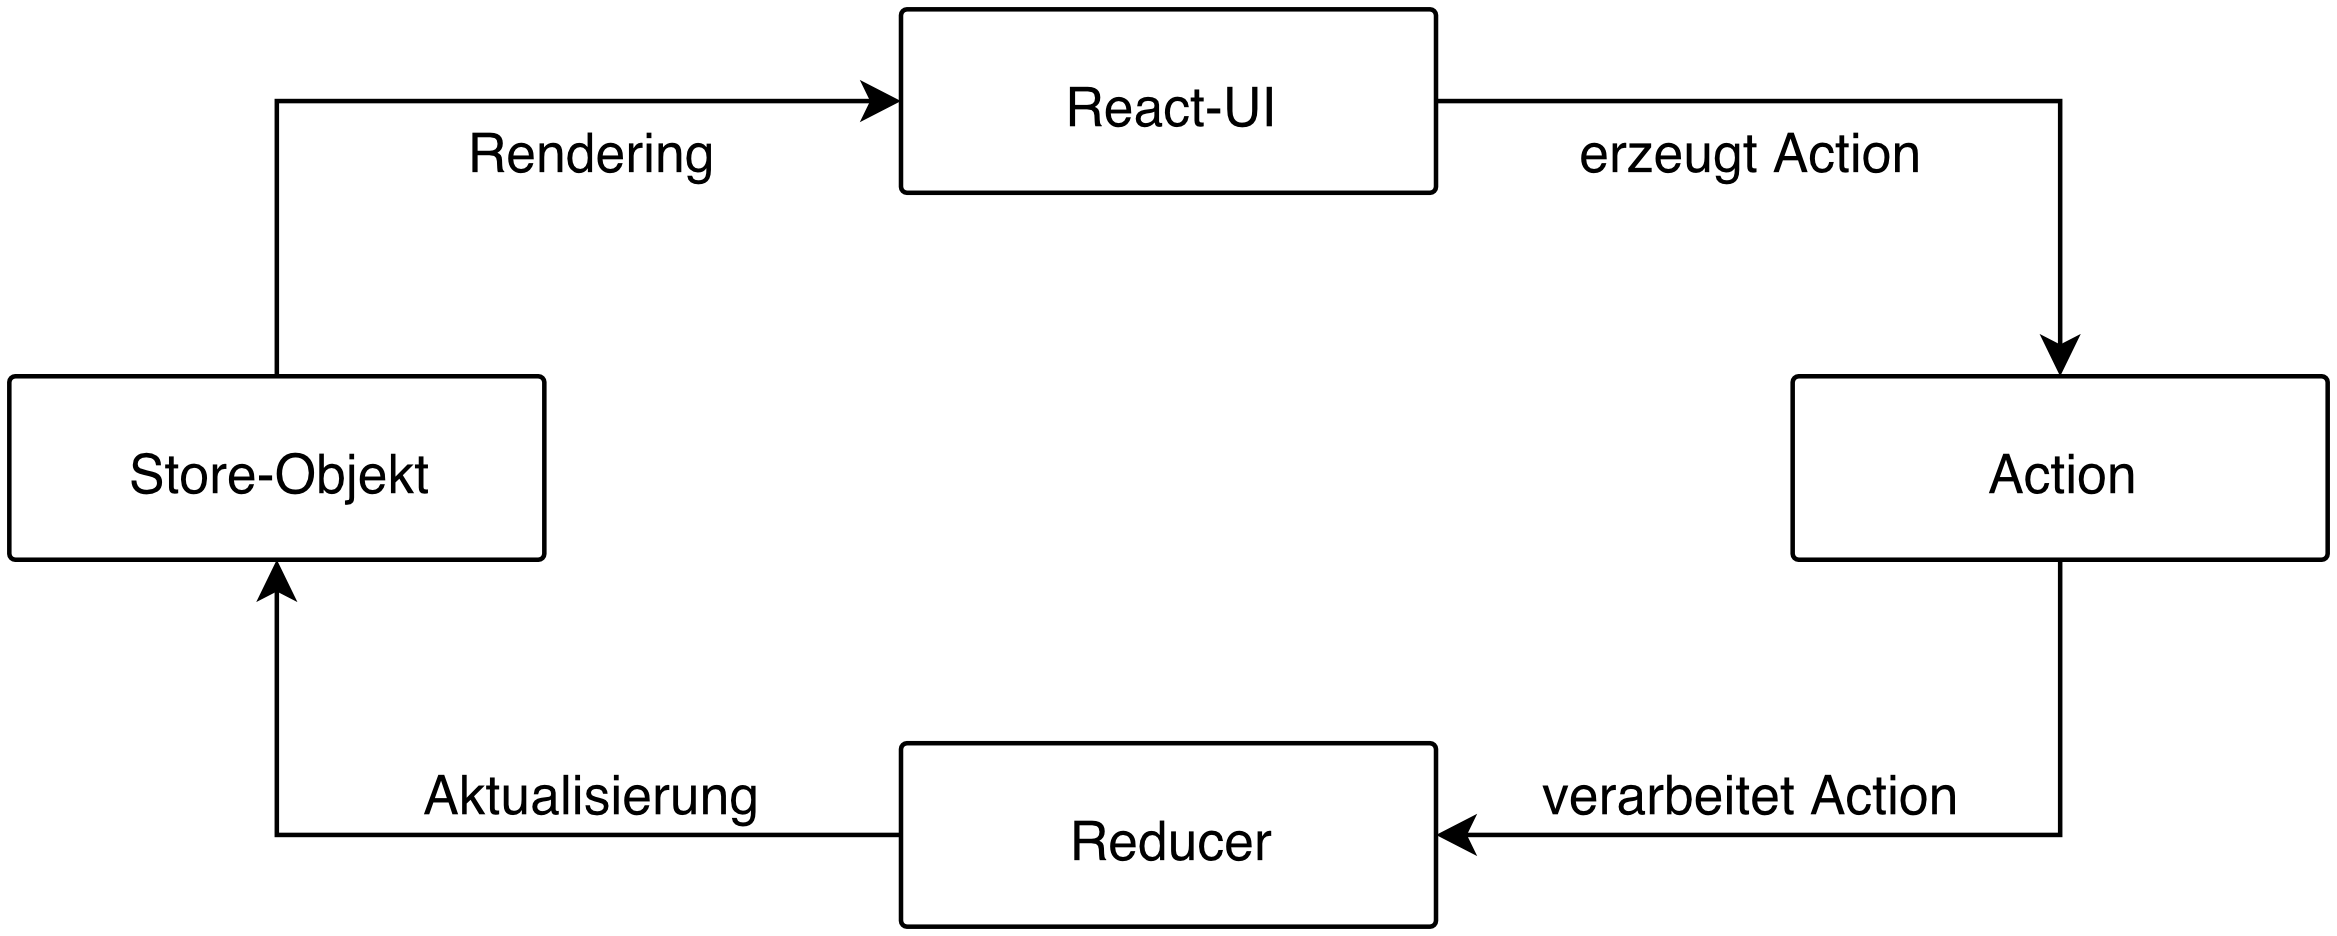
\includegraphics[width=.98\linewidth]{diagrams/ReduxCycle.png}}
\caption[Redux-Zyklus]{der Redux-Zyklus}
\label{figure:ReduxCycle}
\end{figure}
Redux gibt somit einen Kreislauf der Verarbeitung applilaktionsübergreifender Daten vor und bewirkt somit, dass die Darstellung der React-Applikation stets auf dem Store basiert.


\subsection{Jest und Enzyme}
Zum Erstellen von Unit-Tests wird das Testing-Frameworks Jest eingesetzt, da es ebenfalls durch Facebook entwickelt wird und somit höchstmögliche Kompatibilität mit den React-Komponenten bietet. Weiterhin bietet das Framework als Besonderheit die Erstellung von \emph{Snapshot-Tests}, mit deren Hilfe es sehr einfach ist, die korrekt Struktur von großen Objekten, wie das Rendering von React-Komponenten, sicherzustellen \autocite[vgl.][]{Facebook:JestIntroduction}.
Die Tests werden mit dem Kommandozeilenbefehl \emph{jest} ausgeführt.
Beim Ausführen der Tests analysiert Jest das Projekt und erfasst automatisch Test-Dokumente und führt diese aus. 
Die Erfassung der Test-Dokumente kann jedoch auch eingeschränkt werden, indem bei der Ausführung der Tests ein Teil des Dokumentennamen übergeben wird. Dies beschleunigt den Aufruf einzelner Tests. 
Ergänzt wird der Einsatz des Jest-Frameworks durch die Nutzung der Funktionsbibliothek Enzyme. Enzyme wurde speziell für das Testen von React-Komponenten entwickelt und bietet Funktionalitäten, die das Testen von React-Komponenten erleichtern \autocite[vgl.][]{Enzyme:Introduction}.

\subsection{Das SVG-Format}
Das \emph{Scalable Vector Graphics}-Format (SVG) ist eine XML-basierte Markup-Sprache welche eine Vektorgrafik beschreibt. SVG-Grafiken können als *.svg-Dateien gespeichert und innerhalb von HTML-Quelltext platziert werden \autocite[vgl.][]{W3C:AboutSVG}. 

Innerhalb des FreeDesign-Editors wird das SVG-Format für die Produkt- und Designdarstellung, sowie für die Darstellung von Bearbeitungswerkzeugen eingesetzt. 

\subsection{Git}
\label{chap:git}
Zur zentralen Quelltextverwaltung nutzt Unitedprint das Versionsverwaltungssystem Git, welches Dateiänderungen protokolliert und die Änderungen Versionen zuweist. Dadurch ist es möglich jede Änderungen im nachhinein nachzuvollziehen, mit einem vorhergehenden Zustand zu vergleichen und bei Bedarf rückgängig zu machen \autocite[vgl.][]{Git:About}.

Weiterhin bietet Git die Möglichkeit verschiedene Zustände eines Projektes in sogenannten \emph{Branches} zu verwalten, wobei jedes Git-Projekt einen eigenen Haupt-Branch besitzt. Um diesen während der 
Entwicklung nicht zu beeinflussen, können Änderung in eigenen Branches entwickelt werden und nach Abschluss der Entwicklungsarbeit mit dem Haupt-Branch zusammengeführt werden \autocite[vgl.][]{Git:Branching}. 

Git biete eine Vielzahl weiterer Funktionalitäten, um mit Branches zu arbeiten, deren Beschreibung jedoch für das Verständnis der Diplomarbeit nicht notwendig ist. 

Für das zentrale Management von Git-Projekten setzt Unitedprint die Software Bitbucket ein, welches von einem IT-internen Operations-Team verwaltet wird. Über Bitbucket können Entwickler die Integration eines Branches in einen anderen Branch beantragen, was als Pull-Request bezeichnet wird. Pull-Requests können von anderen Entwicklern begutachtet werden und Änderungen am Projektinhalt, die durch das Zusammenführen verursacht würden, kommentiert werden. Weiterhin bietet Bitbucket die Funktionalität sogenannter Pipelines, mit deren Hilfe automatisiert Integrationsschritte ausgeführt werden können \autocite[vgl.][]{Bitbucket:Product}.

Das FreeDesign-Projekt wird in einem eigenem Git-Projekt verwaltet.

% Status: Zweitprüfung
\section{Integration des FreeDesign-Projektes}

\subsection{Veröffentlichungszyklus}
Die Geschäftsführung des Unternehmens gibt einen wöchentlichen Veröffentlichungszyklus für das gesamte Softwaresystem vor, wobei jeden Montag am frühen Morgen eine neue Version veröffentlicht wird. 

Dies wird durch die Anwendung des Paradigmas der kontinuierlichen Integration ermöglicht. 
Das Paradigma wurde durch Kent Beck (\citeyear[59]{Beck2004}) geprägt und beschreibt, dass die Entwickler eines Team regelmäßig Änderungen in die Quelltextbasis integrieren. Nach jeder Integration wird werden automatisiert das ausführen der Unit-Test sowie das Kompilieren der Software durchgeführt. Durch diesen Prozess erhalten die Entwickler ein regelmäßigen Feedback über die Richtigkeit ihrer Entwicklung.

\subsection{Git-Struktur}
Der FreeDesign-Editor für die produktive Anwendung wird auf der Basis des Haupt-Branch namens \emph{master} kompiliert. 
Jeden Montag wird durch die Zusammenführung mit einem \emph{release}-Branch die Veröffentlichung der neuen Version durchgeführt. 
Der \emph{release}-Branch wiederum wird in der Woche zuvor donnerstag Vormittag auf der Basis eines \emph{develop}-Branch erstellt. Neue Funktionalitäten, Fehlerkorrekturen und sonstige Änderungen am Quelltext werden in eigenen Git-Branchen, sogenten \emph{Feature}-Branches entwickelt. Wurde eine Änderung fertiggestellt, wird mit einem \emph{Pull-Request} die Zusammenführung der Änderung in den \emph{develop}-Branch beantragt.
Wurde die Zusammenführung genehmigt und durchgeführt, ist die Änderung somit automatisch Bestandteilt der nächsten Veröffentlichung. 


\subsection{Bereitstellungsablauf}
Vor der Zusammenführung wird jedoch die Änderung intensiv geprüft. Hierfür wird automatisch auf der Basis des \emph{Pull-Requests}
eine Pipeline in Bitbucket ausgelöst. 
Basierend auf der Beschreibung von Silvio Gohl (Operations-Team Unitedprint.com SE) kann der Ablauf der Pipeline wie folgt beschrieben werden.
Zunächst erstellt die Pipeline auf der Basis des Feature-Branch einen temporären Branch, in welchem der Feature-Branch und der \emph{develop}-Branch zusammengeführt werden. 
Die nächsten Schritte der Pipeline sind die Ausführung der Unit-Tests und das testweise Kompilieren des FreeDesign-Editors. Treten bei diesen Schritten Fehler auf, müssen sie durch den Entwickler korrigiert und der Pull-Request neu erstellt werden. 

Verlief das Erstellen des Pull-Request ohne Probleme, werden die anderen Mitglieder des Teams informiert und gebeten eine Begutachtung der Änderungen durchzuführen. Diese haben nun die Möglichkeit die Änderungen in Bitbucket zu begutachten und zu kommentieren. Wurden die Änderungen von mindestens zwei Entwicklern bestätigt, kann der Feature-Branch mit dem develop-Branch zusammengeführt werden. 

Sobald eine Änderung im develop-Branch enthalten ist, steht sie auf einem Testserver zur Verfügung. Die Änderung wird nun von der hausinternen Abteilung für die Qualitätssicherung, sowie von der Fachabteilung, die die Änderung in Auftrag geben hat, überprüft.
% Status: Zweitprüfung
\section{Integrationsprozess der Designvorlagen}
Auf dem Webportal \emph{design.easyprint.com} wird für jedes Produkt nur ein Produktformat zur Gestaltung einer Designvorlage angeboten. Durch einen Integrationsprozess wird die eigenreichte Designvorlage auf die anderen Formate des Produktes sowie auf weitere Produkte adaptiert.

Die Adaptierung führt eine hauseigene Grafikabteilung unter verwendung der Software \emph{Adobe Illustrator}, welche eine Software zur Erstellung von Vektor-Grafiken ist \autocite[vgl.][]{Adobe:Illustrator}. 
Ein Teil der Adaptierungsarbeit ist das Definieren von Text- und Farbschlüsseln, die später im Integrationsprozess durch Übersetzungstexte und Farben der Farbschemen ersetzt werden. 

Die Designvorlagen werden im Anschluss als SVG-Dateien exportiert und durch einen Importprozess in das Easyprint-Shop-System integriert. 
In einem ersten Schritt wird zunächst die SVG-Datei in eine Datenstruktur übersetzt, welche der FreeDesign-Editor einlesen kann. Auf Basis der so entstandenen  
Datenstruktur werden die Sprach/Farb-Derivate erzeugt und auf den Webservern, für die Verwendung im FreeDesign-Editor, gespeichert.  

In einem letzten Schritt wird das 3D-Vorschaubild erzeugt, welches zur Präsentation auf der Übersichtsseite eingesetzt wird. Für das Erzeugen eines Vorschaubildes werden die SVG-Grafiken der Designs der einzelnen Produktseiten verwendet. 
Diese werden in einem Schritt vorher, direkt nach dem Speichern der Sprach/Farb-Derivate erzeugt. Es wird somit für jedes Sprach/Farb-Derivat ein 3D-Vorschaubild erzeugt.
Die Abbildung \ref{fig:Vorlagenimport} stellt den gesamten Integrationsprozess durch ein Aktivitätsdiagramm dar.

\begin{figure}[H]
    \centering
    \includegraphics[width=.98\textwidth]{diagrams/FreeDesign-Vorlagenerstellung.pdf}
\caption{Integrationsprozess der Designvorlagen als Aktivitätsdiagramm}
\label{fig:Vorlagenimport}
\end{figure}

Das FreeDesign-Projekt unterstützt den Integrationsprozess durch die Bereitstellung eines Kommandozeilenprogramms für die automatische Konvertierung der SVG-Dateien in die Datenstruktur für den FreeDesign-Editor. Weiterhin wird ein Kommandozeilenprogramm für die automatische Erzeugung der SVG-Dateien der einzelnen Produktseiten bereitgestellt. Beide Schritte sind in Abbildung \ref{fig:Vorlagenimport} gestrichelt eingerahmt. 

%% TODO: ? \subsection{Software-Architektur}

    % Ergebnisse.tex
\chapter{Ergebnisse}

% Ist-Architektur.tex
\section{Ist-Architektur}

% Status: Erstkorrektur
%%%%%%%%%%%%%%%%
%%% Workshop %%%
%%%%%%%%%%%%%%%%
\subsection{Ergebnis des Workshops zur Ist-Architektur}

\subsubsection{Positives und Erhaltenwertes}
Als positiv wurde hervorgehoben, dass die Architektur, zumindest soweit bekannt, nicht an unlösbaren Problemen leidet. 
Dies war in einer früheren Implementation des FreeDesign-Editors der Fall gewesen.

Auch Anforderungsänderung und Erweiterungen konnten bisher problemlos umgesetzt werden.

Die Nutzung von Redux als zentrale Zustandsverwaltung, sowie das Verbinden des Redux-States an die React-Komponenten über \emph{Container}-Objekte wurde ebenfalls als positiv gewertet. 

Als unbedingt erhaltenswerte wurde auch die strikte Trennung zwischen Produktdarstellung und Designdarstellung, sowie den grafischen Komponenten zur Bearbeitung des Designs bewertet. 

%Die grundlegende Strukturierung des Quelltextes innerhalb der Ordner hat sich ebenfalls bewährt und scheint den Einstieg in das Projekt zu fördern. 
%Mitgliedern des Entwicklerteam ist die Strukturierung auch aus andere Projekte bekannt.

\subsubsection{Schwächen und Probleme}
\paragraph{Die unzureichende Strukturierung der Geschäftslogik}
wurde als schwerwiegendste Schwäche der Architektur kritisiert.
Diese ist an verschiedensten Stellen im Quelltext implementiert. Den Mitgliedern des Teams ist oft während der Entwicklungsarbeit nicht klar, ob eine bestimmte Funktionalität bereits implementiert ist und an welcher Stelle im Quelltext diese zu finden ist. 
Daher wird vermutet, dass einige Funktionalitäten mehrfach implementiert sind. 
Dies verstößt gegen das, durch Dave Thomas und Andy Hunt formulierte Prinzip, \emph{"Don’t Repeat Yourself" (DRY)}. Es besagt, dass jedes Wissen innerhalb eines Systems ein einzige, eindeutige und verbindliche Darstellung haben muss \autocite[vgl.][30 - 31]{ThomasAndHunt2020}. 

Quelltext-Duplikate sind aus mehreren Gründen problematisch. Bei Änderungen, müssen mehrerer Stellen im Quelltext angepasst werden. Neben den Funktionalitäten sind auch Unit-Tests mehrfach implementiert, die das Selbe testen und bei Änderungen angepasst werden müssen. Neben dem höheren Entwicklung- und Wartungsaufwand, führen Duplikate auch zu einer größeren JavaScript-Datei für den FreeDesign-Editor. 

\paragraph{Der Mangel inhaltlicher Konventionen} war ein weiterer Kritikpunkt gewesen. Es bestehen technische Konventionen für die Implementation von Quelltext, jedoch mangelt es an fachlichen und inhaltlichen Konventionen. Die Konventionen die in der Ist-Architektur bestehen, resultieren aus der Verwendung von TypeScript, ReactJS und Redux. Beispiele hierfür sind, dass React-Komponenten keine Geschäftslogik enthalten und die Verwendung von \emph{Container}-Objekten zum Verbinden von \emph{React}-Komponenten und \emph{Redux}.
Diese Konventionen wurden jedoch nicht schriftlich festgellegt, sonden bestehen aus mündlichen Absprachen. 
% Darüberhinaus wurden keine Konventionen für den fachlichen und strukturellen Inhalt des Quelltextes festgellegt. 
% Das führt unter anderem dazu, dass es kein Schema für die Bezeichnung von Klassen, Funktionen oder Modulen gibt. Weiterhin werden Funktionen teilweise in Klassen und teilweise in Modulen zusammen gefasst. 

\paragraph{Die Strukturierung der Kommandozeilenprogramme} für die Integration der Designvorlagen wurde ebenfalls kritisiert, welche innerhalb des Editor-Projekt implementiert sind.
Es fällt den Teammitgliedern  schwer, bei Quelltextkomponenten die von den Kommandozeilenprogramme genutzt werden, zu unterscheiden, ob diese exklusiv für die Kommandozeilenprogramme bestehen oder nicht. Dadurch besteht die Gefahr, dass Änderungen der Kommandozeilenprogramme unbeabsichtigt den FreeDesign-Editor mit ändern. Dies verlangsamt die Entwicklungsarbeit und erhöht den Testaufwand.

Die TypeScript-Datei \lstinline|draftImporterCli.ts| welche das Kommandozeilenprogramme zur Konvertierung der Adobe-Illustrator-Dateien enthält, liegt innerhalb des Ordners \lstinline|src|. Für das Kommandozeilenprogramme zum Konvertieren der FreeDesign-Designstruktur in SVG-Dateien ist die Datei \lstinline|designToSvgConverter.ts| im Ordner \lstinline|src/designToSvgCLI| verantwortlich. Diese Strukturierung der Programme wurde als inkonsistent empfunden. 
Es wurde durch das Team angeregt, innerhalb des \lstinline|src|-Ordner einen Ordner ein für Kommandozeilenprogramme zu etablieren, in dem die beiden Programme enthalten sind. Desweiteren wurde vorgeschlagen, dass diese Ordner sämtlichen Quelltextkomponenten enthalten, die exklusiv durch die Kommandozeilenprogramme genutzt werden.  

\paragraph{Das Verwenden generischer Ordner}, welche in Listing \ref{list:genericdirs} angeben sind, wurde durch das Team bemängelt und führt oft zu Unklarheiten. Für die \lstinline|common|-Ordner bestand kein klarer Grund dafür, dass diese zusätzlichen Ebenen geschaffen wurden. Es bestand nur die diffuse Idee, häufig genutzte Komponenten in diesen Ordnern zu sammeln. 

\begin{lstlisting}[language={sh}, label=list:genericdirs, caption=generische Ordner die innerhalb des FreeDesign-Projektes genutzt werden]
src/actions/helper
src/components/common
src/containers/common
src/core/common
src/core/helpers
src/utils
\end{lstlisting}

Carola Lilienthal empfiehlt das Vermeiden von generischen Hilfklassen, da sie von überall her benutzt werden können und die Zusammenarbeit mit anderen Klassen nicht einschränkt wird \autocite[vgl.][159]{Lilienthal2019}. 

Die selben Argumentation liese sich auch das Verwenden generischer Ordnername anwenden. 
% Mit der selben Begründung sollte auch das Verwenden von Ordnern wie \emph{helper}, \emph{common} oder \emph{utils} vermieden werden. Diese Ordner dienen als Sammelorte für Module, deren Zuordnung unklar ist oder für Hilfs-Module. 


% Status: Zweitkorrekt
\subsection{Analyseergebnis der obersten Ordnerebene}
\subsubsection{Übersicht der obersten Ordnerebene}
\label{sec:overview}
Die Quelltextdateien, welche die Anwendungen beschreiben, sind innerhalb des Ordners \lstinline|src| organisiert. 
% Die obersten Ordnerebene des \emph{src}-Ordner spiegelt die Architektur der Anwendung auf höchster Ebene wider.
Abbildung \ref{fig:obersteOrdnerebene} stellt die funktionalen Zusammenhänge der obersten Ordnereben innerhalb des Ordners als Abhängigkeitsgraph dar.  
% Wird innerhalb eines Ordners Quelltext aus einem benachbarten Ordner importiert, wird dies durch eine Pfeilspitze am benachbarten Ordner gekennzeichnet. Beispielsweise importiert Quelltext innherhalb des Ordners \lstinline|designToSvgCLI| Quelltext aus dem Ordner \lstinline|core|.
\begin{figure}[H]
	\centering
    \caption{Übersicht der obersten Ordnerebene innherhalb des Ordner \lstinline|src|}
	\label{fig:obersteOrdnerebene}
	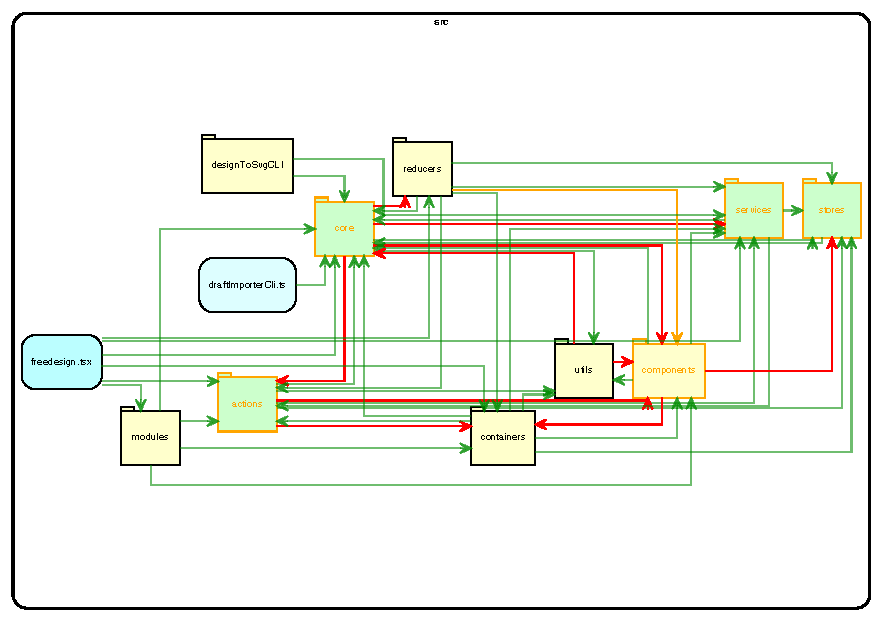
\includegraphics{diagrams/Ist-Architektur/Projektuebersicht.pdf}
\end{figure}


Der Abhängigkeitsgraph zeigt sämtliche Ordner die im Ordner \lstinline|src| enthalten sind, so wie die TypeScript-Dateien \lstinline|freedesign.tsx| und \lstinline|draftImporterCli.tsx|, die ebenfalls im Ordner \lstinline|src| hinterlegt sind.  

Durch die Pfeile werden die Abhängigkeiten der Komponenten gekennzeichnet. Die Pfeilspitze zeigt auf den Ordner, auf dessen Inhalt Zugriffe erfolgen. Beispielsweise greift Quelletext im Ordner \lstinline|designToSvgCLI| auf Quelletext aus dem Ordner \lstinline|core| zu.
Wird eine Abhängigkeit durch das \lstinline|allowed|-Array bestätigt, wird diese durch einen grünen Pfeil dargestellt. Eine Abhängigkeit die durch das \lstinline|forbidden|-Array erfasst wird, wird durch einen roten Pfeil gekennzeichnet. Wird eine Abhängigkeit durch keine der beiden Arrays erfasst, wird diese durch einen orangen Pfeil dargestellt.

Enthält ein Ordner ungenutzten Quelltext, wird dies durch einen orangen Rahmen und einer orangen Bezeichnung gekennzeichnet.

\subsubsection{Ordnerinhalt der obersten Ordnerebene}
\paragraph{Der Ordner \emph{core}} ist für den Anwendungskern vorgesehen und enthält Geschäftslogik sowie grundlegende Funktionalitäten und Datenstrukturen der Anwendung. 
Es ist vorgesehen, dass umgebender Quelletext auf den Quelltext des \lstinline|core|-Ordners zugreifen darf, jedoch ist der Zugriff aus dem \lstinline|core|-Ordner heraus auf den umgebenden Quelletext untersagt. Dem Ordner mangelt es an einer klaren Strukturierung, auf Grund deren die richtige Zuordnung und das Auffinden der Geschäftslogik schwierig sind. 

\paragraph{Im Ordner \emph{components}} sind React-Komponenten zur Erzeugung der grafischen Oberfläche enthalten. Darunter zählen Komponenten zur Erzeugung von Menüs, Dialogen oder auch Werkzeuge zu Designbearbeitung. Die Komponenten besitzen keine Verbindung zum \emph{Redux-State} und rufen keine \emph{Redux-Actions} auf. Die Komponenten können bei der Verwendung mit Eigenschaften versehen werden und damit an Redux gebunden werden. Dadurch ist das Verwenden der React-Komponenten in unterschiedlichen Kontexten möglich.

\paragraph{Der Ordner \emph{containers}} enthält Komponenten (Container-Komponenten), welche die \emph{ReactJS}-Komponenten aus dem Ordner \lstinline|components| mit den \emph{Redux-State} sowie \emph{Redux-Actions} verbindet. Somit verbinden die Container-Komponenten die grafische Oberfläche der Anwendung mit Redux.

% Ein Beispiel hierfür ist der \emph{Container} \lstinline|LoginDialog.tsx|, welcher das Anmeldeformular für die Kundenanmeldung erzeugt. Dieser nutzt Formularelemente und Schaltflächen aus dem \emph{components}-Ordner zur Erzeugung der grafischen Oberfläche. Für die Prüfung, ob der Kunden erfolgreich angemeldet ist, greift der Dialog auf die Kundendaten zu, die im \emph{Redux-State} verwaltet werden. Über eine \emph{Redux-Action} wird die Anmeldung durchgeführt, welche vom \emph{Container} aufgerufen wird. Dadurch das die grafischen Formularelement und Schaltflächen nicht an den Anwendungszustand gebunden sind, konnten sie z.B. auch in einem Dialog zur Kundenregistrierung verwendet werden.


\paragraph{Die Ordner \emph{reducers}, \emph{action} und \emph{stores}} beziehen sich auf Redux und enthalten die Redux-Reducer, die Redux-Actions sowie den Redux-State. Der Redux-States ist auf mehrere Dateien innerhalb des Ordners \lstinline|stores| aufgeteilt. Die Dateien beziehen sich auf unterschiedliche Teile der Anwendung. Beispielsweise wird der Zustand der grafischen Oberfläche in der Datei \lstinline|guiState.ts| verwaltet und der Zustand des Designs, welches gestaltet wird, in der Datei \lstinline|productState.ts| verwaltet. 

\paragraph{Der Ordner \emph{services}} enthält, zusätzlich zu den Redux-Actions \lstinline|ApiActions.ts| im Ordner \lstinline|actions|,  Quelletext zur Kommunikation mit der Unitedprint-API. Außerdem endhält er Quelletext zur Kommunikation mit der Zwischenablage des Betriebssystems, wodurch das Kopieren und Einfügen von Texten beim Bearbeiten eines Designs ermöglicht wird.

% Für die Kommunikation mit der API von Unitedprint wird das Modul \emph{redux-axios-middleware} eingesetzt. 
% Das Module ist eine \emph{Redux}-Middleware für die asynchrone HTTP-Kommunikation. HTTP-Anfragen werden durch den Aufruf von \emph{Redux-Actions} ausgelöst, ebenso werden \emph{Redux-Actions} nach eintreffender Antwort ausgelöst \autocite[vgl.][]{ReduxAxios}. Im Ordner \emph{services} sind die \emph{Redux-Actions} für die API-Aufrufe definiert. Desweiteren enthält der Ordner noch eine Serviceklasse zur Kommunikation mit Zwischenablage des Betriebssystems. Die Klasse ermöglicht das einfügen von Text aus der Zwischenablage in das Design, sowie das Kopier von Text aus dem Design in die Zwischenablage.

\paragraph{Im Ordner utils} befinden sich nur zwei TypeScript-Dateien. Wie bereits im Architektur-Workshop festgestellt, ist die Existenz dieses Ordners fragwürdig und sollte durch die Soll-Architektur aufgelöst werden.  

\paragraph{Der Ordner \emph{modules}} wird ebenfalls durch die Soll-Architektur aufgelöst, da er React- und Redux-Komponenten enthält, welche in die Ordner \lstinline|components| und \lstinline|containers| integriert werden können.

\paragraph{Im Ordner \emph{styles}} sind globalen \emph{CSS}-Definitionen untergebracht, die das optische Erscheinungsbild der Anwendung beschreiben. Die Definitionen werden ausschließlich Komponenten im Ordner \emph{components} verwendet. 

\paragraph{Der Ordner \emph{designToSvgCLI}} enthält das Kommandozeilenprogramm für die Design-SVG-Konvertierung im Integrationsprozess der Designvorlagen, welche im Abschnitt \ref{sect:Integrationsprozess_Designvorlagen} beschrieben wurde.


\paragraph{}Die TypeScript-Datei \lstinline|freedesign.tsx| ist die Startdatei des FreeDesign-Editors, über die das Programm gestartet wird. Für das Kommandozeilen-Programm zum Import der AI-Dateien, welches ebenfalls in Abschnitt \ref{sect:Integrationsprozess_Designvorlagen} beschrieben wurde, ist die Datei \lstinline|draftImporterCli.ts| als Startdatei vorgesehen.


% \paragraph{Zugriffe}
% Die grünen Zugriffspfeile stellen erwartete Zugriffe dar und sind somit gewollte Kopplungen der Einzellkomponenten. Im Gegensatz dazu sind die roten und orangen Zugriffspfeile ungewollte Zugriffe und wurden mit der Zeit integriert. Bei den roten Zugriffen besteht außerdem das Problem, dass diese Zyklen erzeugen und damit gegen die Forderung an eine Architektur, zyklusfrei zu sein, verstoßen. 

% Es bestehe sowohl einzelne Zyklen, wie zwischen den Ordner \emph{core} und \emph{services} sowie Zyklengruppen. Ein Beispiel hierfür ist die Gruppe bestehend aus \emph{actions}, \emph{utils} und \emph{core}.
% Auch innerhalb der Ordner bestehe Zyklen wischen Unterkomponenten. 
% Insgerammt wurden 14 Zyklen festgestellt.

% \paragraph{Verwaister Quelltext}
% Innerhalb der orange gekennzeichneten Ordner befinden sich verwaiste Quelltextabschnitte, welche nicht aufgerufen werden. Solche Quelltextstellen können die Verständlichkeit des Quelltext einschänken. 


% \begin{figure}[H]
% 	\centering
% 	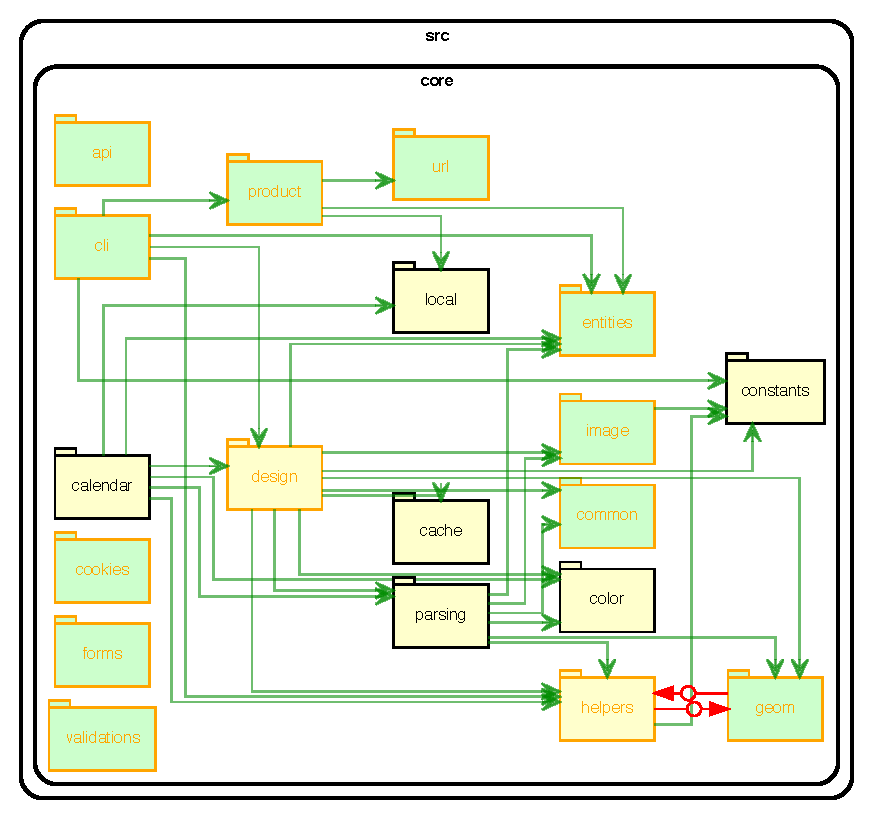
\includegraphics{diagrams/Ist-Architektur/core-graph.pdf}
% 	\caption{Übersicht  }
% 	\label{fig:coreGraph}
% \end{figure}


% Produktdarstellung.tex
\subsection{Produktdarstellung}
Eine zentrale Komponenten der Anwendung ist die Darstellung einer Produktseite, welche auf dem \textit{SVG}-Format basiert.
Das SVG-Format ist eine XML-basiertes Markup-Sprache welche eine zweidimensionale Grafik beschreibt und innherhalb von HTML-Quelltext platziert werden kann \autocite[vgl.][]{AboutSVG}. 

Wie von Abbildung \ref{fig:Produktdarstellung} zu entnehmen ist, werden für das Erzeugen der \textit{SVG}-Struktur \textit{ReactJS}-Komponenten genutzt, die exklusiv für die Produktdarstellung erstellt wurden. Diese Komponenten finden in keinem anderem Zusammenhang Verwendung und sind eng an die Produktdarstellung gekoppelt. 
Zur Darstellung des Produktes gehören das Darstellen von Beschnittlinien, Falzlinien, Nutlinien, Bereichen die nicht bedruckbar sind, sowie Seitenbezeichnungen. Bei einigen Produkten, Textilien oder Werbeprodukte, kann im Hintergrund eine Abbildung des Produktes dargestellt werden. Die Komponente \textit{SVGPageRenderer} ist für verantwortlich für die Produktdarstellung und wird Komponente \textit{PagePresenter.tsx} eingesetzt. Diese wiederum ist für Präsentation des Produktes innerhalb des FreeDesign-Editors verantwortlich und ermöglicht das Rotieren, Skalieren sowie das Verschieben der Darstellung. 


Das Produkt wird durch eine Struktur beschrieben, welche im \textit{core}-Ordner hinterlegt ist. Die Struktur enthält sowohl geometrische Information für die Produktdarstellung, als auch Produktspezifische eigenschaften, wie die Existenz von Beschnittlinien. 

Für die Darstellung innerhalb des FreeDesign-Editors ist die Nutzung von mathematischen Operationen notwendig, die im Anwendungskern definiert sind. 

\begin{figure}[H]
    \centering
    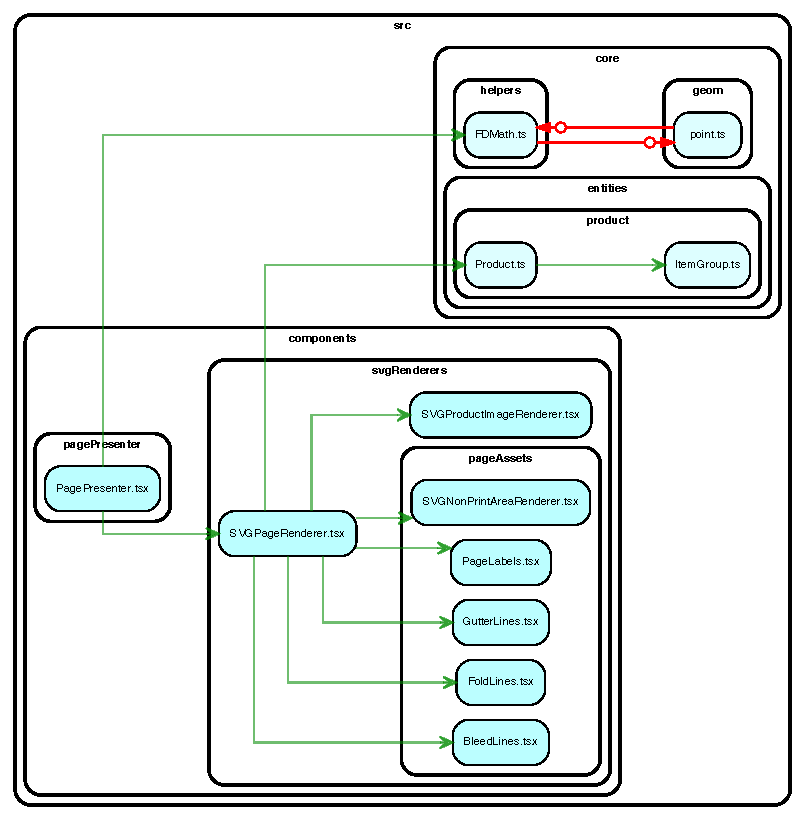
\includegraphics{diagrams/Ist-Architektur/page-presenter-analysis.pdf}
    \caption{Abhängigkeiten der Komponenten für Produktdarstellung}
    \label{fig:Produktdarstellung}
\end{figure}

Der Produktdarstellung kann ein Kindelement übergeben werden, welches in die die Produktdarstellung eingebettet werden. 

\lstinputlisting[frame=single,label=beispielcode,caption=Quelletext-Bsp.: Designdarstellung eingebettet Kindelement]{sourcecode/product.tsx}

\input{chapter/ergebnisse/Ist-Architekur/Komponenten/Komponenten-Produktdarstellung.tex}
% Status: Erstkorrektur
% Designdarstellung.tex

\subsection{Designpräsentation}
Die Designpräsentation basiert ebenfalls auf dem SVG-Format, welche durch die React-Komponente \lstinline|DesignPresenter.tsx| erzeugt wird. 

Die Designpräsentation wird der Produktpräsentation als Kindkomponente übergeben. Dadurch sind beiden React-Komponenten voneinander entkoppelt und das Design wird lediglich innerhalb der Produktdarstellung dargestellt.

Die Abbildung \ref{fig:Designdarstellung} weißt die Abhängigkeiten der Designpräsentation auf.

\begin{figure}[H]
    \centering
    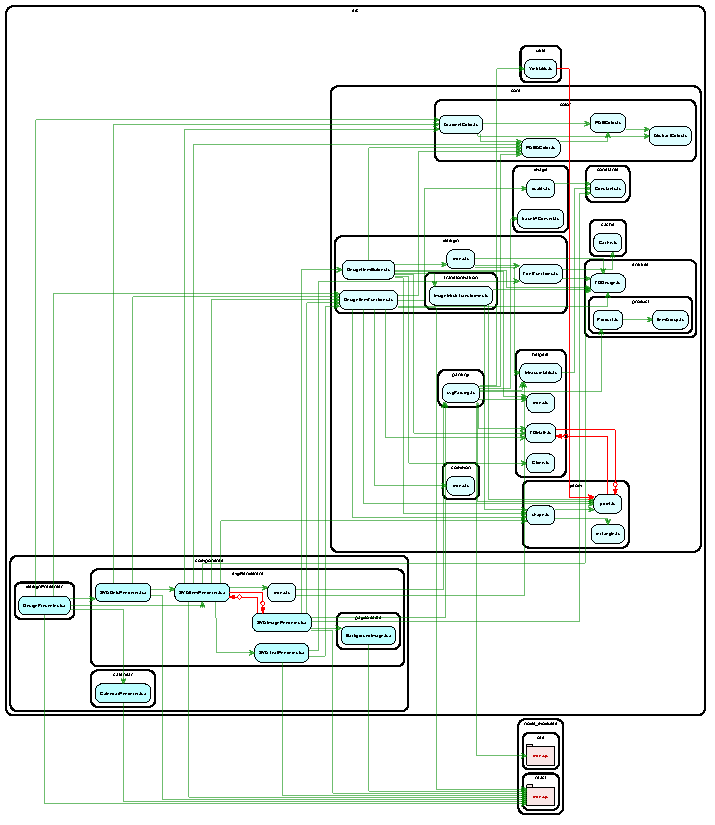
\includegraphics{diagrams/Ist-Architektur/design-presenter-analysis.pdf}
    \caption{Abhängigkeiten der Komponenten für Designdarstellung}
    \label{fig:Designdarstellung}
\end{figure}

Die Designpräsentation ist von einige Datenstrukturen und Funktionalen der \lstinline|core|-Komponente abhängig. 

Folgende Bausteine wurden aus den Abhängigkeiten extrahiert.
\begin{multicols}{2}
\input{chapter/ergebnisse/Ist-Architekur/Komponenten/Komponenten-Designdarstellung.tex}
\end{multicols}
% Designbearbeitung.tex
\subsection{Designbearbeitung}
Die dritte Hauptkomponente des FreeDesign-Editors ist das bearbeiten des Designs. Hierfür stellt der Editor Eingabekomponenten zur Verfügung, welche Änderungen der Designstruktur im \textit{Redux-State} bewirken. Auf diese Änderungen reagiert die Designdarstellung und löst eine Aktualisierung aus, wodurch keine Abhängigkeiten zwischen der Darstellung des Designs und der Bearbeitung des Designs bestehen. Beide Komponenten greifen lediglich auf die selbe Designstruktur zu.  
Die \textit{Container}-Komponente \textit{Stage.tsx} verbindet alle Komponenten, die für die Bearbeitung des Designs Notwendig sind. Hierzu gehören grafisch Komponente zur Darstellung von Auswahlrahmen, eine Texteingabe sowie Hilfswerkzeugen, wie einem Lineal oder einem Gitter. 
Desweiteren ist sie mit dem \textit{Redux-Store} verbunden und ruft sie verschieden \textit{Redux-Actions}. 
Mit  1260 Quelltextzeilen, 51 Funktionen und 46 Importen, handelt es sich um die komplexeste Komponente des FreeDesign-Editor und kann als eine \textit{Man-in-the-middle-Klasse} bezeichnet werden. Hierbei handelt es sich um ein Antimuster bei dem eine Klasse zu viele zuständigkeiten hat \autocite[vgl.][619]{Geirhos2015}.
Im allgemeinen ist der Quelltext und die Abhängigkeiten für die Designbearbeitung sehr komplex und ungenügend strukturiert. Das bearbeiten eines Designs ist die Kernfunktionalität des FreeDesign-Editor und sollte von einer Soll-Architektur aus der restlichen Anwendung als entkoppelte Komponente extrahiert werden. 
% GUI.tex
\subsection{Grafische Oberfläche}
Die grafische Oberfläche bindet den Baustein zum Designbearbeitung und damit auch die Bausteine Design- und Produktdarstellung ein. Um diese Bausteine herum sind verschiedenste grafische Elemente integriert, die das Bearbeiten des Design unterstützen, sowie die Produktkonfiguration. Außerdem sind Elemente zur steuern  und visualisieren von Kundendaten enthalten, wie das Speicher und Öffnen von Designentwürfen oder die Anzeige des Warenkorbs.
Die Abhängigkeiten der grafischen Oberfläche sind sehr komplex und sind in der Darstellung \emph{D3\_Grafische\_Oberfläche.html} visualisiert. 

Die grafische Oberfläche ist auch das volatilste Element des FreeDesign-Editors und unterliegt ständiger Änderungen und Erweiterungen. Basierend auf Martin (\citeyear[119]{Martin2018}) sollte der volatile Teile eines Quelltext von stabilen Teile isoliert werden. Gerade im Quelltext für die Bereitstellung der Funktionalitäten zu Verschieben, Rotieren und Skalieren von Designobjekt besteht die Gefahr, dass Änderungen der Grafischen Darstellung dem stabile Quelltext für Objekt-Transformationen beschädigt. 
Folgende Bausteine der grafischen Oberfläche wurden identifiziert.

\begin{multicols}{2}    
    \input{chapter/ergebnisse/Ist-Architekur/Komponenten/Komponenten-GUI.tex}
\end{multicols}
\subsection{Kommandozeilenprogramm Adobe-Illustrator-Designkonvertierung}

\begin{figure}[H]
    \centering
    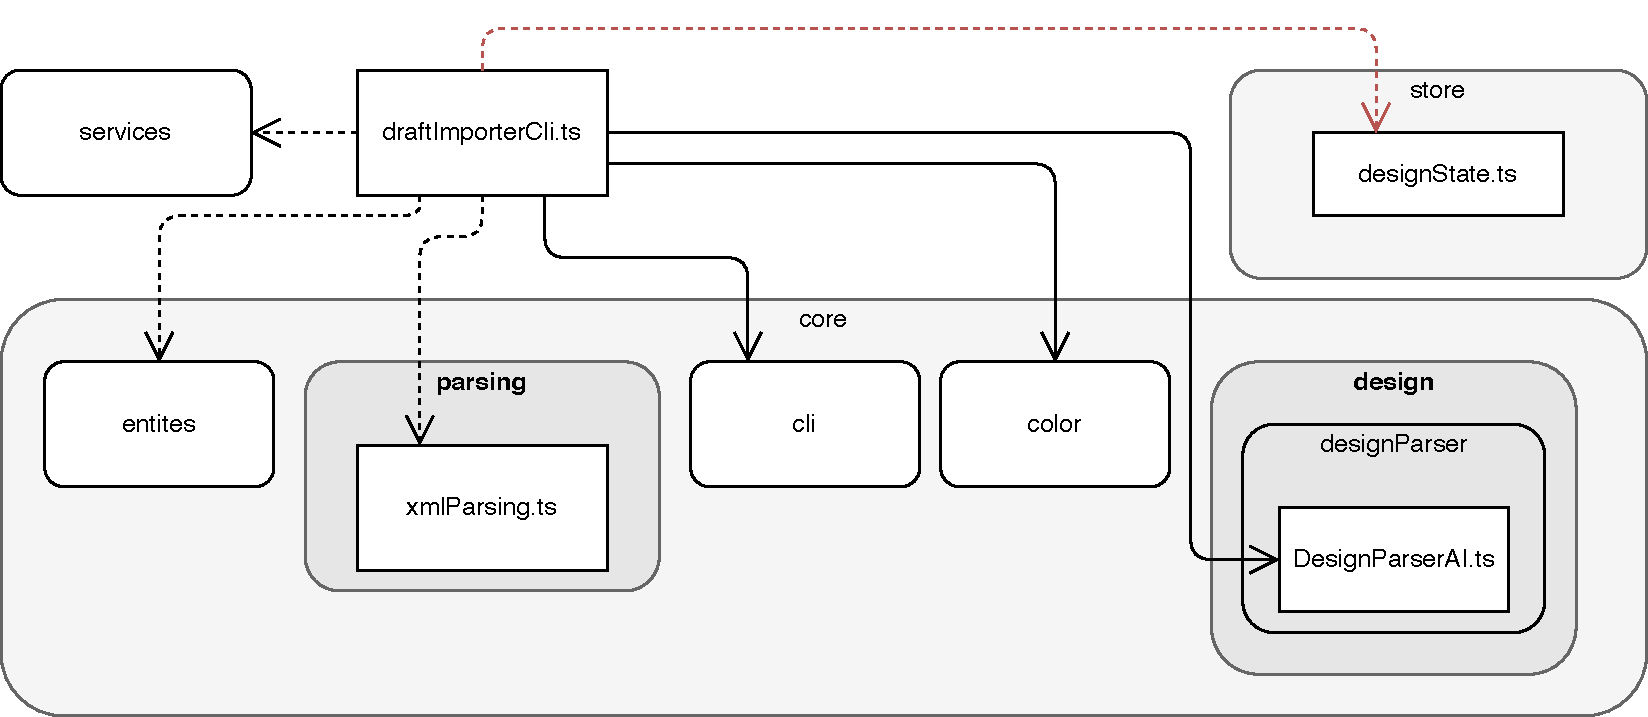
\includegraphics{diagrams/Ist-Architektur/draftImporter-analysis.pdf}
    \caption{Abhängigkeiten der Komponenten für das Kommandozeilenprogramm zur Konvertierung von Designs die mit Adobe-Illustrator erstellt wurden zu FreeDesign-Designs.}
    \label{fig:DesignImport}
\end{figure}

\begin{multicols}{2}    
    \input{chapter/ergebnisse/Ist-Architekur/Komponenten/Komponenten-DesignImport.tex}
\end{multicols}
\subsection{Kommandozeilenprogramm Design-SVG-Konverter}
Nach der, in Kapitel \ref{Kommandozeilenprogramm Adobe-Illustrator-Designkonvertierung} \emph{Kommandozeilenprogramm Adobe-Illustrator-Designkonvertierung} beschrieben, Konvertierung der Designvorlagen, werden Derivate der Vorlagen erzeugt. Diese enthalten übersetzte Texte, für die unterschiedlichen Sprachen in denen die Vorlagen angeboten werden. Um die Vielfalt der Vorlagen zu erhöhen, werden außerdem weitere Derivate mit unterschiedlichen Farbzuordnung erzeugt. Die Erzeugung der Derivate ist nicht Bestandteil des FreeDesign-Projektes. Jedoch werden in einem letzten Prozessschritt 3D-Vorschaubilder der Derivate zur Präsentation im Webshop erzeugt. Die Erzeugung der Vorschaubilder, die ebenfalls nicht Teil des FreeDesign-Projektes ist, basiert auf SVG-Dateien die durch das FreeDesign-Projektes erzeugt werden. Hier zu 


Konvertierung der Designvorlagen, werden in einem weiteren Prozessschritt 3D-Vorschaubilder für die Präsentation im Webshop erzeugt. 

Das FreeDesign-Projekt unterstützt den, im Kapitel \ref{Kommandozeilenprogramm Adobe-Illustrator-Designkonvertierung} \emph{Kommandozeilenprogramm Adobe-Illustrator-Designkonvertierung} beschrieben, Import der Designvorlagen durch ein weiteres Kommandozeilenprogramm. 

\begin{figure}[H]
    \centering
    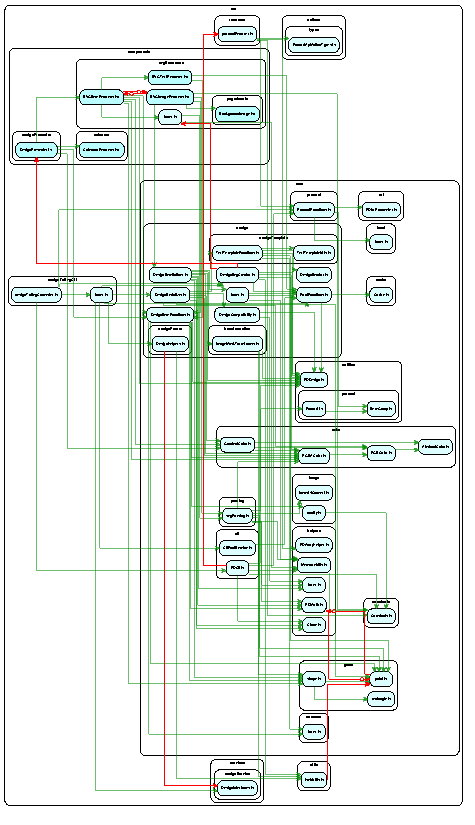
\includegraphics{diagrams/Ist-Architektur/designToSvgCLI-analysis.pdf}
    \caption{Abhängigkeiten der Komponenten für das Kommandozeilenprogramm zur Konvertierung von Designs zu SVG-Dateien.}
    \label{fig:DesignToSvg}
\end{figure}
\begin{multicols}{2}
    \input{chapter/ergebnisse/Ist-Architekur/Komponenten/Komponenten-DesignToSvg.tex}
\end{multicols}
\subsection{Zusammenfassung der Ist-Architektur}
% Auf fehlendes SOLID eingehen
% Übersicht der Quelltextzuordnung im Anhang

\section{Soll-Architektur}
\subsection{Ergebnis des Workshops zur Soll-Architektur}
% 
\subsection{Entwurf einer optimierten Soll-Architektur}
Entwurf einer Soll-Architektur, die die Schwächen der Ist-Architektur ausmerzt.

\subsection{Prototyp}
Implementation der Soll-Architektur in einem Prototypen zur Bestätigung der Machbarkeit.

\section{Migrationsstrategie}
\subsection{Migrationsschritte}
Ausarbeitung von Migrationsschritten die zum Erreichen der Soll-Architektur notwendig sind.

\subsection{Priorisierung}
Priorisierung der Migrationsschritte.

\subsection{Migrationsplan}
Erstellung eines Ablaufplans zu Migration.

\subsection{Vorgehensweise für das Refactoring}
Beschreibung einer Vorgehensweise wie das Refactoring für die einzelnen Migrationsschritte vorgenommen werden sollte.
=> Test-Abdeckung, Separieren von Quelltext, etc.

    % Diskussion.tex

%TODO: Diskussion
%TODO: Auf fehlendes SOLID eingehen
%TODO: Keine Kohesion in common Ordnern
%TODO: Ansätze von Smart-UI
%TODO: Ist-Architektur eher Package by Layer-Architektur auf oberste eben => Package by component darunter
% Architekturworkshop => unterschiedlich gute Motivation der Teammitglieder
% Analyse Ist-Architektur  => es wurden Artefakte in Quelltext eingeführt

%\paragraph{Kritik }
%Eine gute Architektur zeichnet sich, basierend auf Robert C. Martin ([vgl.][S. 196 - 197]{Martin2018}), dadurch aus, dass sie keine Vorgaben über die verwendete Technologien macht und offen gebgenüber Technologieänderungen ist. 
%Diese wird von der aktuellen Architektur auf der obersten Ordnerebene nicht erfüllt. Würde z.B. ein Technologwechsel zur Verwaltung des Anwendungszustands durchgeführt werden, würde das einen Änderung der Architektur bedeuten.

% Mit  1260 Quelltextzeilen, 51 Funktionen und 46 Importen, handelt es sich um die komplexeste Komponente des FreeDesign-Editor und kann als eine \emph{Man-in-the-middle-Klasse} bezeichnet werden. Hierbei handelt es sich um ein Antimuster bei dem eine Klasse zu viele zuständigkeiten hat \autocite[vgl.][619]{Geirhos2015}.

%
%Der aktuellen Architektur wurde zum Zeitpunkt ihrer Entwicklung kein Architekturmuster zugrunde gelegt, was viel Raum zu Interpretation der Architektur lässt. 

% TODO: Diskussion Aufteilung der Redux-Files
% TODO: Es war schwierig Diagramme zu erstellen, da keine klasse / interfaces

% TODO: auf Quelltextleichen eingehen

% \paragraph{Testbarkeit} 
% TODO: Bei Änderung des Quelltextbasis müssen sowohl der FreeDesign-Editor als die Kommandozeilenprogramme getestet werden, auch wenn die Änderung nur ein Programm betrifft.


%TODO: \paragraph{Gefahr von Quelltextleichen}
%% Unter Quelltextleichen ist Quelltext zu verstehen, der nicht ausgeführt wir \autocite[vgl.][292]{Martin2009}. Sollte das Importieren von Designvorlagen nicht mehr notwendig sein oder es wird ein alternativer Prozess gefunden, existiert weiterhin Quelltext im FreeDesign-Projekt, der das Projekt aufbläht und aufwändig entfernt werden sollte.

    \subsection{Zusammenfassung der Ist-Architektur}
% Auf fehlendes SOLID eingehen
% Übersicht der Quelltextzuordnung im Anhang
    % Ausblick.tex
\chapter{Ausblick}
% TODO: Ausblick
% Analyse auf aktuellen Projektstand analysieren


    \printbibliography[heading=bibintoc, title={Quellenverzeichnis}]

    % TODO: Eidesstattliche Erklärung
    % TODO: Eidesstattliche Erklärung ohne Nummerierung
    % TODO: Anlagen
\end{document}
